\subsection{Figuras Planas}
\subsubsection{Congruencia y Semejanza}
Se dice que dos ángulos son congruentes si tienen la misma medida.

De la misma forma, dos segmentos de recta son congruentes si miden lo mismo. \\

Por extensión, dos figuras planas son llamadas \textbf{congruentes} si tienen \textbf{exactamente} la misma forma y tamaño, es decir, si y solo si, todos sus ángulos interiores y lados son congruentes entre sí.
En este contexto, entre dos figuras, los vértices, lados y ángulos que coinciden (homologamente) son llamados \textbf{correspondientes}. La congruencia entre objetos se denota "$\cong$".

Por el otro lado, dos figuras son \textbf{semejantes} ($\sim$) si tienen la misma forma, pero no necesariamente el mismo tamaño (la congruencia es una clase de semejanza), es decir, si todos sus ángulos interiores correspondientes son iguales y la razón entre las medidas de sus lados es constante.\\
\subsubsection{Triángulos}
\textbf{Criterios de Congruencia}\\
\textit{Lado, Lado, Lado (LLL)}: Todos los lados respectivos son congruentes entre ellos.\\
\textit{Lado, Ángulo, Lado (LAL)}: Dos lados respectivos son congruentes, al igual que el ángulo comprendido entre ellos.\\
\textit{Ángulo, Lado, Ángulo (ALA)}: Dos ángulos respectivos son congruentes, al igual que el lado entre ellos.\\

\textbf{Criterios de Semejanza}\\
\textit{Ángulo, Ángulo (AA o AA)}: Todos los ángulos son iguales entre ellos (con dos basta por las propiedades de un triángulo).\\
\textit{Lado, Ángulo, Lado (LAL)}: Dos lados tienen medidas \textbf{proporcionales} y los ángulos comprendidos entre ellos son congruentes.\\
\textit{Lado, Lado, Lado (LLL)}: Todos los lados correspondientes son \textbf{proporcionales}, es decir hay una constante para la relación entre cada par de lados.\\

\textbf{Teorema de Euclides}\\
En un triángulo \textbf{rectángulo}, la altura de la hipotenusa divide al triángulo en dos triángulos semejantes entre ellos, al igual que semejantes al triángulo original. De esto se deriva que el cuadrado de tal altura es igual al producto entre las protecciones de los catetos sobre la hipotenusa:
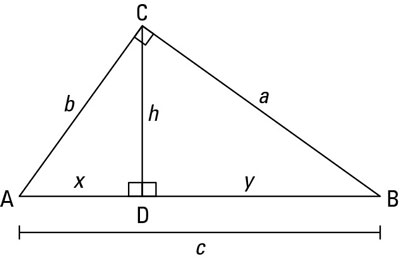
\includegraphics[width=\columnwidth]{euclides.jpg}
\begin{equation*}
{h_c}^2 = x \cdot y
\end{equation*}
También de esto se deriva que el cuadrado de un cateto es igual al producto de la hipotenusa y su proyección del cateto.

\begin{equation*}
    a^2 = c \cdot y; b^2 = c \cdot x
\end{equation*}
\textbf{Teorema de Pitagoras}\\
En un triángulo \textbf{rectángulo}, el área del cuadrado construido sobre la hipotenusa es igual a la suma de las áreas de los cuadrados sobre los catetos.
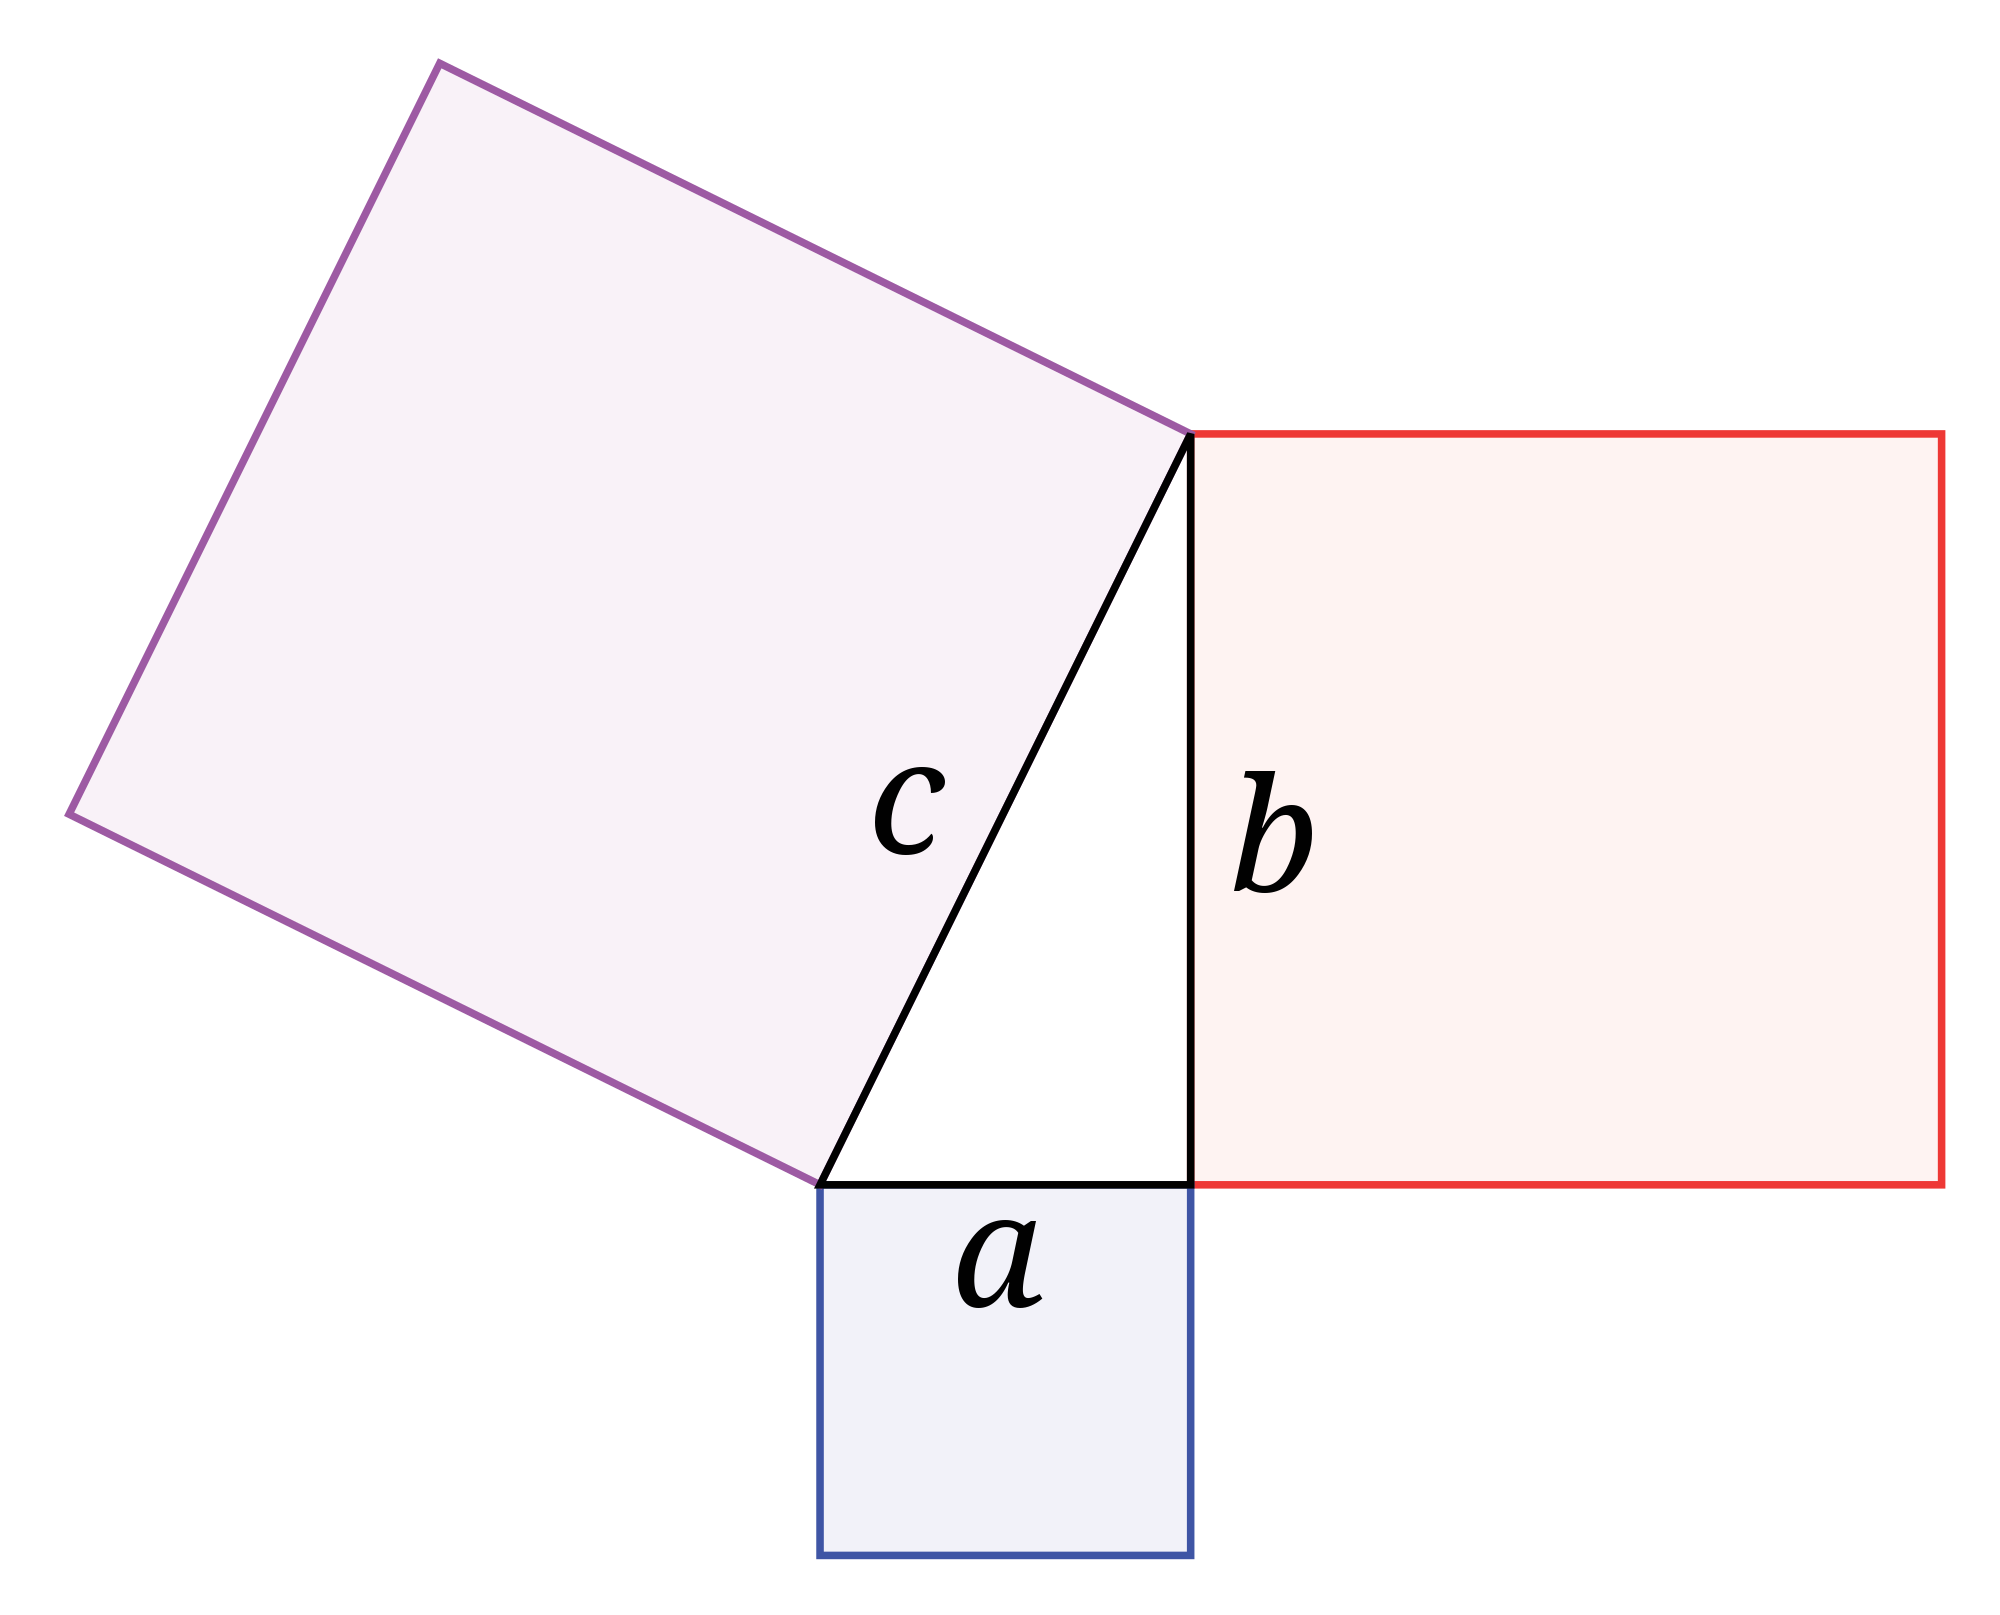
\includegraphics[width=\columnwidth]{pitagoras.png}

De esto deriva la \textbf{ecuación pitagórica}:
\begin{equation*}
    a^2 + b^2 = c^2
\end{equation*}
Es importante notar que esta es un teorema \textbf{recíproco}, es decir, cuando esta ecuación se cumple en un triángulo dado se puede afirmar que es rectángulo.\\
